% SPDX-License-Identifier: CC-BY-SA-4.0
% Author: Matthieu Perrin
% Part: 
% Section: 
% Sub-section: 
% Frame: 

\begingroup

\begin{frame}{Point vocabulaire}

  \begin{tabular}{ccc}
    &Une seule unité d'exécution & Plusieurs unités d'exécution
    \\
    
\begin{tikzpicture}
      \draw[white] (0, 0) rectangle (2,3);
      \draw (1, 1.75) node{Problème};
      \draw (1, 1.25) node{Séquentiel};
    \end{tikzpicture}
    &
    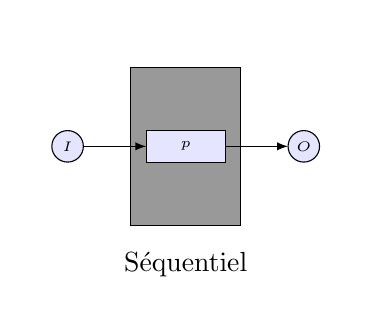
\begin{tikzpicture}

      \draw[white] (-0.5, -0.3) rectangle (3.5,3);
      \draw (1.5, 0) node{Séquentiel};

      \draw[fill=black!40] (0.8, 0.5) rectangle (2.2,2.5);
      \draw[fill=blue!10] (1.5, 1.5) +(-0.5, -.2) rectangle +(0.5, .2) +(0,0) node{\tiny $p$};

      \draw[-latex] (0.2, 1.5) -- (1,1.5);
      \draw[-latex] (2, 1.5) -- (2.8,1.5);

      \draw[fill=blue!10] (0, 1.5) circle (2mm) node{\tiny $I$};
      \draw[fill=blue!10] (3, 1.5) circle (2mm) node{\tiny $O$};
    \end{tikzpicture}
    &
    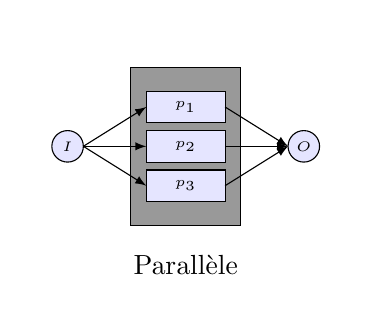
\begin{tikzpicture}
      \draw[white] (-0.5, -0.3) rectangle (3.5,3);
      \draw (1.5, 0) node{Parallèle};

      \draw[fill=black!40] (0.8, 0.5) rectangle (2.2,2.5);
      \draw[fill=blue!10] (1.5, 2) +(-0.5, -.2) rectangle +(0.5, .2)   +(0,0) node{\tiny $p_1$};
      \draw[fill=blue!10] (1.5, 1.5) +(-0.5, -.2) rectangle +(0.5, .2) +(0,0) node{\tiny $p_2$};
      \draw[fill=blue!10] (1.5, 1) +(-0.5, -.2) rectangle +(0.5, .2)   +(0,0) node{\tiny $p_3$};

      \draw[-latex] (0.2, 1.5) -- (1,2);
      \draw[-latex] (0.2, 1.5) -- (1,1.5);
      \draw[-latex] (0.2, 1.5) -- (1,1);

      \draw[-latex] (2, 2)   -- (2.8,1.5);
      \draw[-latex] (2, 1.5) -- (2.8,1.5);
      \draw[-latex] (2, 1)   -- (2.8,1.5);

      \draw[fill=blue!10] (0, 1.5) circle (2mm) node{\tiny $I$};
      \draw[fill=blue!10] (3, 1.5) circle (2mm) node{\tiny $O$};
    \end{tikzpicture}
    \\
    
\begin{tikzpicture}
      \draw[white] (0, 0) rectangle (2,3);
      \draw (1, 1.75) node{Problème};
      \draw (1, 1.35) node{de};
      \draw (1, 0.95) node{concurrence};
    \end{tikzpicture}
    &
    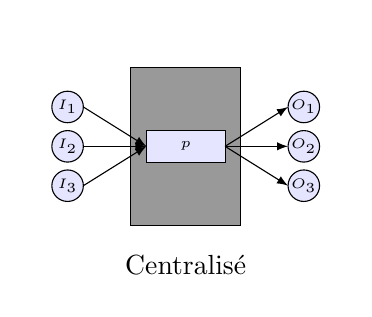
\begin{tikzpicture}
      \draw[white] (-0.5, -0.3) rectangle (3.5,3);
      \draw (1.5, 0) node{Centralisé};

      \draw[fill=black!40] (0.8, 0.5) rectangle (2.2,2.5);
      \draw[fill=blue!10] (1.5, 1.5) +(-0.5, -.2) rectangle +(0.5, .2) +(0,0) node{\tiny $p$};

      \draw[-latex] (0.2, 2) -- (1,1.5);
      \draw[-latex] (0.2, 1.5) -- (1,1.5);
      \draw[-latex] (0.2, 1) -- (1,1.5);

      \draw[-latex] (2, 1.5) -- (2.8,2);
      \draw[-latex] (2, 1.5) -- (2.8,1.5);
      \draw[-latex] (2, 1.5) -- (2.8,1);

      \draw[fill=blue!10] (0, 2) circle (2mm)   node{\tiny $I_1$};
      \draw[fill=blue!10] (0, 1.5) circle (2mm) node{\tiny $I_2$};
      \draw[fill=blue!10] (0, 1) circle (2mm)   node{\tiny $I_3$};

      \draw[fill=blue!10] (3, 2) circle (2mm)   node{\tiny $O_1$};
      \draw[fill=blue!10] (3, 1.5) circle (2mm) node{\tiny $O_2$};
      \draw[fill=blue!10] (3, 1) circle (2mm)   node{\tiny $O_3$};
    \end{tikzpicture}
    &
    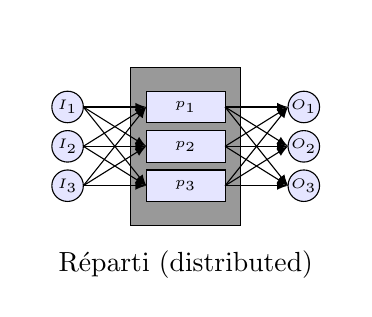
\begin{tikzpicture}
      \draw[white] (-0.5, -0.3) rectangle (3.5,3);
      \draw (1.5, 0) node{Réparti (distributed)};

      \draw[fill=black!40] (0.8, 0.5) rectangle (2.2,2.5);
      \draw[fill=blue!10] (1.5, 2) +(-0.5, -.2) rectangle +(0.5, .2)   +(0,0) node{\tiny $p_1$};
      \draw[fill=blue!10] (1.5, 1.5) +(-0.5, -.2) rectangle +(0.5, .2) +(0,0) node{\tiny $p_2$};
      \draw[fill=blue!10] (1.5, 1) +(-0.5, -.2) rectangle +(0.5, .2)   +(0,0) node{\tiny $p_3$};

      \draw[-latex] (0.2, 2) -- (1,2);
      \draw[-latex] (0.2, 2) -- (1,1.5);
      \draw[-latex] (0.2, 2) -- (1,1);

      \draw[-latex] (0.2, 1.5) -- (1,2);
      \draw[-latex] (0.2, 1.5) -- (1,1.5);
      \draw[-latex] (0.2, 1.5) -- (1,1);
      
      \draw[-latex] (0.2, 1) -- (1,2);
      \draw[-latex] (0.2, 1) -- (1,1.5);
      \draw[-latex] (0.2, 1) -- (1,1);

      \draw[-latex] (2, 2)   -- (2.8,2);
      \draw[-latex] (2, 2)   -- (2.8,1.5);
      \draw[-latex] (2, 2)   -- (2.8,1);
      
      \draw[-latex] (2, 1.5) -- (2.8,2);
      \draw[-latex] (2, 1.5) -- (2.8,1.5);
      \draw[-latex] (2, 1.5) -- (2.8,1);
      
      \draw[-latex] (2, 1)   -- (2.8,2);
      \draw[-latex] (2, 1)   -- (2.8,1.5);
      \draw[-latex] (2, 1)   -- (2.8,1);

      \draw[fill=blue!10] (0, 2) circle (2mm)   node{\tiny $I_1$};
      \draw[fill=blue!10] (0, 1.5) circle (2mm) node{\tiny $I_2$};
      \draw[fill=blue!10] (0, 1) circle (2mm)   node{\tiny $I_3$};

      \draw[fill=blue!10] (3, 2) circle (2mm)   node{\tiny $O_1$};
      \draw[fill=blue!10] (3, 1.5) circle (2mm) node{\tiny $O_2$};
      \draw[fill=blue!10] (3, 1) circle (2mm)   node{\tiny $O_3$};
    \end{tikzpicture}
  \end{tabular}

\end{frame}

\endgroup
\endinput
